\chapter{Gauge potentials in time-dependent media}
\label{chapter:theory}

From the previous chapter, the generation of a synthetic gauge \textit{field} relies completely on the presence of a synthetic gauge \textit{potential} which arises from the existence of non-reciprocal phases. Creating these phases for light invariably requires breaking reciprocity. Here, it is shown that the influence of the velocity field on light in a moving medium can be formulated in terms of a gauge potential, which will lead to observable measurements of a direction-dependent phase. The more constrained case of a potential arising from the motion of water in both a linear waveguide and surrounding a rotating cylinder dielectric will then be shown to act as an effective magnetic potential for light, introducing a non-reciprocal phase that can be exploited to demonstrate an optical analogue to the Aharonov-Bohm effect. This phase can also be generated through dynamic modulation of a waveguide, and the gauge potential emerging from such modulations is derived based on the work of Fang et al. \cite{Fang2012}.

\section{Moving media}

To show how a moving media forms an effective vector potential for light, first consider the curl components of Maxwell's equations for moving media without sources \cite{Mansuripur2009a},

\begin{align} 
	\nabla \times \bm{E} &= -\dfrac{\partial \bm{B}}{\partial t}, \label{mwell3}\\
	\nabla \times \bm{H} &= \dfrac{\partial \bm{D}}{\partial t} \label{mwell4}.
\end{align}

Let $\bm{v(r)}$ represent the velocity field associated with the motion of a medium of refractive index $n$, moving along $v \hat{x}$. Then, by taking a first order approximation of the Minkowski relations \ref{HMinkowski} and \ref{DMinkowski}, where $\textbf{v}/c \ll 1$,

\begin{align}
	\bm{B} &= \mu \bm{H} - (n^2 - 1) \dfrac{\bm{v}}{c^2} \times \bm{E}, \\
	\bm{D} &= \epsilon \bm{E} + (n^2 - 1) \dfrac{\bm{v}}{c^2} \times \bm{H}.
\end{align}

These relations allow us to rewrite the curl components of Maxwell's equations in the form

\begin{align}
\nabla \times \bm{E}  -\dfrac{\partial}{\partial t} \Big[(n^2 - 1) \dfrac{\bm{v}}{c^2} \times \bm{E}\Big] &=-\dfrac{\partial}{\partial t}(\mu\bm{H}), \label{a2}\\
\nabla \times \bm{H}  -\dfrac{\partial}{\partial t} \Big[(n^2 - 1) \dfrac{\bm{v}}{c^2} \times \bm{H}\Big] &=-\dfrac{\partial}{\partial t}(\epsilon\bm{E}). \label{a1}
\end{align}

To solve these equations explicitly, we shall assume the light in the media to be a monochromatic plane wave with electric and magnetic fields defined as 

\begin{equation}
\begin{bmatrix}
\bm{E}(\bm{r},t) \\
\bm{H}(\bm{r},t)
\end{bmatrix}
=
\begin{bmatrix}
\bm{E}(\bm{r}) \\
\bm{H}(\bm{r}) 
\end{bmatrix}
e^{-i \omega t},
\label{eqn:planewave}
\end{equation}

which simplifies equations \ref{a2} and \ref{a1} to

\begin{equation}
\Big(\nabla + i \omega (n^2 - 1) \dfrac{\boldsymbol{v}}{c^2}\Big) \times 
\begin{bmatrix}
\bm{E} \\
\bm{H}
\end{bmatrix}
=
i\omega
\begin{bmatrix}
\mu \bm{H} \\
-\epsilon \bm{E}
\end{bmatrix}.
\label{a3}
\end{equation}

To elucidate the relationship between the quantum and classical approach used here, Equation \ref{a3} is multiplied by $-i \hbar$, where $\hbar$ is Planck's reduced constant to obtain

\begin{equation}
(\hat{p} + q \bm{v} ) \times 
\begin{bmatrix}
\bm{E} \\
\bm{H}
\end{bmatrix} 
= 
\hbar \omega
\begin{bmatrix}
\mu \bm{H} \\
-\epsilon \bm{E}
\end{bmatrix} .
\label{eqn:finalfield}
\end{equation}

Straight-away, the quantum momentum operator can be identified: $\hat{p} = -i \hbar \nabla$, as well as the effective charge for the photon in the medium,

\begin{equation}
q =\dfrac{\hbar \omega}{c^2}  (n^2 - 1).
\label{effectiveCharge}
\end{equation}

This charge, $q$, forms the \textit{effective} charge for the light in the medium. Furthermore, the relationship between the gauge potential $\bm{A}$ and flow vector $\bm{v}$ of the medium as simply

\begin{equation}
\bm{A(r)} = \bm{v(r)}.
\end{equation}

This result shows that a relative movement introduced in a medium can be formulated in terms of an effective vector potential, along with an associated `charge' for the light in the medium. 

\subsection{Non-reciprocal phase from a Fizeau-like apparatus}

\begin{figure}[t]
	\centering
	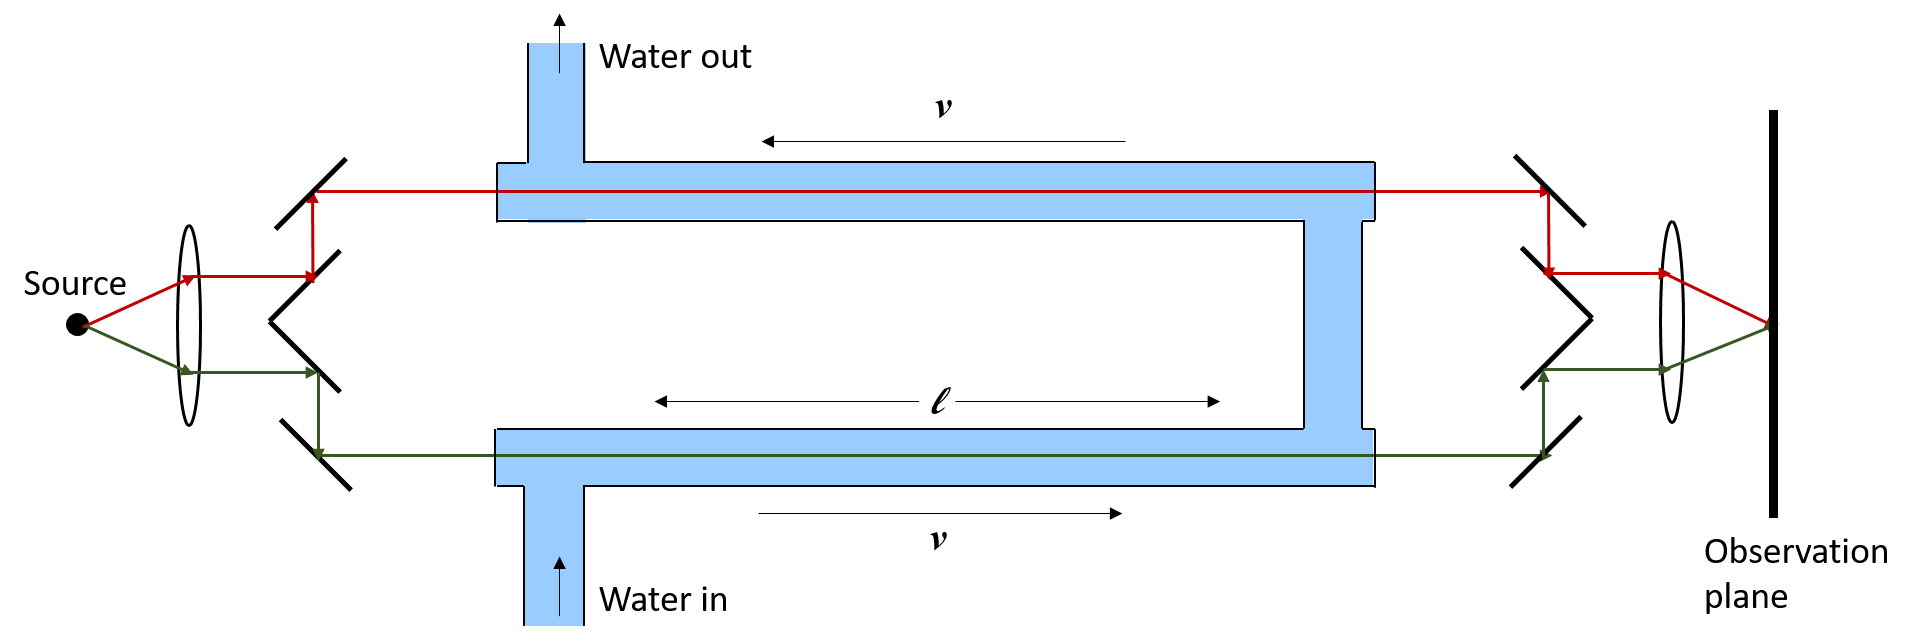
\includegraphics[width=\textwidth]{figures/fizeau.png}
	\caption[The standard apparatus for the Fizeau experiment]{A traditional form of the Fizeau experiment. A source of light is split into two beams, propagating with and against the flow vector of the water respectively. The dragging of the light by the medium forms a non-reciprocal phase, which can be observed by the resulting interference pattern.}
	\label{fig:fizeau}
\end{figure}


Now, consider what happens if a photon were to flow through a medium moving with a linear velocity along $x$, as depicted in Figure \ref{fig:fizeau}. To derive the phase shift it will gain, we will begin with Maxwell's equations from \ref{mwell3} to \ref{mwell4}. Rearranging the magnetic field intensity and displacement field, yields

\begin{align}
\nabla \times \bm{E} &= -\dfrac{\partial \bm{B}}{\partial t}, \label{mwell2_3}\\
\nabla \times \bm{B} &= \mu \epsilon \dfrac{\partial \bm{E}}{\partial t}.
\end{align}

Taking the curl of \ref{mwell2_3} yields,

\begin{equation}
\nabla \times (\nabla \times \bm{E}) = \nabla \times (-\dfrac{\partial \bm{B}}{\partial t}) = -\dfrac{\partial}{\partial t}(\epsilon \mu \dfrac{\partial \bm{E}}{\partial t}),
\end{equation}

where the divergence of the $\bm{E}$ field is $0$, reducing the above equations to the three dimensional Cartesian form of the electromagnetic wave equation,

\begin{equation}
\label{3dwave}
\big(\dfrac{n^2}{c^2} \nabla ^2 - \dfrac{\partial{^2}}{dt^2}\big)\bm{E} = 0.
\end{equation}

Equation \ref{3dwave} transforms under the appropriate Lorentz boost along $v\hat{x}$, defined in Appendix \ref{lorentz} as

\begin{equation}
\Big[1-\big(\dfrac{nv}{c}\big)^2 \Big] \nabla ^2 \bm{E} - \dfrac{2}{c^2} (n^2 - 1) \bm{v} \cdot \nabla \dfrac{\partial E}{\partial t} + \Big[\dfrac{v^2-(nc)^2}{c^4} \Big] \dfrac{\partial ^2 E}{\partial t^2} = 0.
\end{equation}

When the medium is moving slowly with respect to $c$ we can assume $v/c \ll 1$, then the above equation further reduces to the more manageable form

\begin{equation}
\label{boost3dwave}
\nabla ^2 \bm{E} - \dfrac{2}{c^2} (n^2 - 1) \bm{v} \cdot \nabla \dfrac{\partial E}{\partial t} - \dfrac{n^2}{c^2} \dfrac{\partial ^2 \bm{E}}{\partial t^2} = 0.
\end{equation}

Again assuming a monochromatic plane wave solution (\ref{eqn:planewave}) Equation \ref{boost3dwave} reduces to

\begin{equation}
\label{wavey}
\nabla ^2 E - 2i\dfrac{w^2}{c^2}(n^2-1)\dfrac{\bm{v}}{c} \cdot \nabla E + (n\dfrac{w}{c})^2 E = 0.
\end{equation}

Now, recall the time-independent Schr\"odinger equation for an electron in some potential $\bm{A(r)}$ \cite{Sakurai1995},

\begin{equation}
\dfrac{1}{2m} \Big(\dfrac{h}{i} \nabla - \dfrac{e}{c} \bm{A} \Big)^2 \psi = E \psi
\end{equation}

which can be expanded out to give

\begin{equation}
\label{schrod}
\nabla^2 \psi - \dfrac{ie}{\hbar c} \big[ \bm{A} \cdot \nabla \psi + (\nabla \cdot \bm{A}) \psi \big] + \big(\dfrac{2mE}{\hbar^2} + \dfrac{e^2}{\hbar^2 c^2} \bm{A}^2 \big) \psi = 0.
\end{equation}

By visual inspection alone, it is evident that equations \ref{schrod} and \ref{wavey} share a similar form in the low velocity regime to the first order, identical to our result in the previous section. To show this, consider the mapping of \ref{schrod} to the following relations; $\psi \rightarrow E$, $\bm{A} \rightarrow \bm{v}/c$, $e/\hbar c \rightarrow k(n^2-1)$, and $2mE/\hbar^2 \rightarrow (nk)^2$, from which

\begin{equation}
\nabla^2 E - ik(n^2-1) \big[ \dfrac{v}{c} \cdot \nabla E + (\nabla \cdot \dfrac{v}{c})E \big] + \big(n^2k^2 + (k(n^2-1))^2 \dfrac{v}{c} \big) E = 0.
\end{equation}

Which, in the first order approximation of $\textbf{v}/c$ becomes Equation \ref{wavey}. Now, the known solution of the above expanded Schr\"odinger solution is simply
\begin{equation}
\psi(\bm{r}) = \psi_0 \exp \Big[\dfrac{ie}{\hbar} \int_{}^{s(\bm{r})} \bm{A(r')} \cdot d\bm{s'} \Big],
\end{equation}
for a line integral over any path such that the final point $s(\bm{r}) = \bm{r}$ and the curl of $\bm{A}$ is vanishing. 

The interference between two phases traversing different paths is then
\begin{equation}
\Delta \varphi = \dfrac{q}{\hbar} \Big(\int_{P_1} \bm{A} \cdot d\bm{s} - \int_{P_2} \bm{A} \cdot d\bm{s} \Big),
\end{equation}

whereby application of Stoke's theorem,

\begin{equation}
\Delta \varphi = \dfrac{q}{\hbar} \int \nabla \times \bm{A} \cdot \hat{n}\textbf{dS},
\end{equation}

which is the quantum AB effect for electrons. It is evident that this is also a solution for the interference of \ref{wavey}, where the electromagnetic vector potential $\bm{A}$ is replaced with $\bm{v}$,

\begin{equation}
\varphi = \dfrac{w}{c^2} (n^2-1) \int_{S}^{} \nabla \times \bm{v} \cdot d\bm{S}.
\end{equation}
 
If the velocity of the medium in both arms of the Fizeau apparatus is assumed to be uniform, then we can assume $\nabla \times \bm{v} = 0$ for both propagation paths of length $l$. In this case the interference term becomes

%\varphi &= \dfrac{\omega}{c^2} \int_{}^{} 0 \cdot \hat{n} dr \\
\begin{equation}
\varphi = \dfrac{\omega}{c^2} (n^2-1) (2 v l).
\end{equation}

Thus we see that not only does a moving media form a synthetic gauge potential for photons, but that such a potential imparts \textit{direction dependent} phases on the light in question.

\subsection{Photonic Aharonov-Bohm effect for a rotating dielectric}

The potential is not constrained to exist only for linear motion. Here, it is shown that the rotation of a medium is sufficient to mimic the Aharonov-Bohm effect for light. The rotation of the medium forms an effective field that is synonymous with the rotation of the magnetic vector potential. In fact, the curl of the rotation itself gives rise to a gauge field, exactly how the magnetic field is the manifestation of the curl of the magnetic potential ($\bm{B} = \nabla \times \bm{A}$).

Consider first a dielectric cylinder of radius $R$, rotating with an angular velocity $\Omega \hat{z}$ while submerged in a uniform medium of constant viscosity as in Figure \ref{fig:abvieira}. Light traversing the medium will be shown to attain a non-reciprocal phase that is dependent on the radius and angular velocity of the dielectric, despite no interactions with the dielectric taking place. In the Aharonov-Bohm effect, the potential mediates interactions with the field. Here, the rotation of the medium instead mediates interactions with the dielectric cylinder \cite{Vieira2014a}.

\begin{figure}[t]
	\centering
	\def\svgwidth{0.6\textwidth}
	\begin{normalsize}
		\input{figures/RotatingCylinder.pdf_tex}
	\end{normalsize}
	\caption[A rotating medium analogue of the Aharonov-Bohm effect for light]{Proposed rotating cylinder for demonstrating an optical AB effect. A beam of photons is split into 2 paths, $P_1$ and $P_2$ of radius $b$, propagating around a rotating cylinder of angular frequency $\Omega$ immersed in a viscous medium. The light acquires a positive or negative phase depending on whether it is propagating with or against the rotation, leading to an optical AB phase.}
	\label{fig:abvieira}
\end{figure}

The angular velocity imparted to the medium is proportional to the distance from the cylinder. In cylindrical coordinates ($r, \theta, z$) the velocity of the cylinder and the surrounding medium is separated into two regions. One, for the inside of the cylinder ($0\leq r \leq R$), and another for the medium surrounding the cylinder ($r>R$).

\begin{equation}
\bm{v}(r) = 
\begin{cases}
\Omega r \hat{\theta}, & 0\leq r \leq R  \\
\dfrac{\Omega R^2}{r} \hat{\theta}, & r > R.
\end{cases}
\end{equation}

As such, there are two effective potentials dependent on the rotation of the cylinder. The effective field that the photon `feels' is then	

\begin{equation}
\bm{H} = \nabla \times \bm{v} = 
\begin{cases}
\Omega \hat{z}, & 0\leq r \leq R  \\
0, & r > R.
\end{cases}
\end{equation}

As expected, the effective field $\bm{H}$ is only non-vanishing inside the cylinder. Likewise, similar to electromagnetic fields, a vanishing of the magnetic field does not imply that the potential is also $0$. In fact, the vector potential is not uniquely defined, since any number of arbitrary curl-free components can be added without changing the effective field. As long as the cylinder is rotating at a constant angular velocity, the strength of the effective field as `felt' by the photon is independent of the position inside the cylinder.

Now, consider a light source propagating through the uniform medium surrounding the cylinder with respect to an observer in the rest frame (Fig \ref{fig:abvieira}. Surrounding the rotating cylinder, it has been shown that despite the effective magnetic field vanishing, an effective gauge potential of $\frac{\Omega R^2}{r} \hat{\theta}$ remains. Suppose that the packet of light is split into two separate paths of radius $b$, with path 2 ($P_1$) propagating in the direction of rotation, and path 1 ($P_2$) propagating along the opposite direction. In propagating along these paths, the wave-function of the light acquires a phase,

\begin{equation}
\phi_{1,2} = \dfrac{q}{\hbar} \int_{P_{1,2}}^{} \boldsymbol{A} \cdot d\boldsymbol{r}.
\end{equation}

So that the relative phase shift of the light along the paths $P_1$ and $P_2$, which both share the same initial and final points, is given by

\begin{equation}
\Delta \phi = \dfrac{q}{\hbar} \int_{P_1}^{} \boldsymbol{A} \cdot d\boldsymbol{r} - \dfrac{q}{\hbar} \int_{P_2}^{} \boldsymbol{A} \cdot d\boldsymbol{r} = \dfrac{q}{\hbar} \oint  \boldsymbol{A} \cdot d\boldsymbol{r}.
\end{equation}

An important distinction to make in the above equations is that they are independent of the time taken to traverse the closed path. In other words, a photon moving at close to the speed of light will acquire exactly the same phase as a photon travelling significantly slower.
Upon substitution of appropriate quantities, where $q$ is the effective charge of the photon derived in Equation \ref{effectiveCharge},

\begin{equation}
\phi = \dfrac{\omega}{c^2}(n^2 - 1) \int_{0}^{2\pi} \frac{\Omega R^2}{b} \hat{\theta} \cdot b d\theta \hat{\theta}.
\end{equation}

Explicitly calculating this phase difference yields the result

\begin{equation}
\phi = \dfrac{2 \pi \omega}{c^2} (n^2 - 1) \Omega R^2,
\end{equation}

where $n$ is the refractive index of the medium. That is, the phase difference of the interfering light is dependent on several properties of the dielectric cylinder. This result is exceedingly similar to the result for the linearly moving medium. The water still plays the same role as that of an effective potential, however the vorticity is no longer vanishing, and represents instead the effective field of the medium.

It is important to reiterate that both these processes are strictly non-reciprocal. Consider instead injecting photons from the right-hand side and measuring interference at the left. The photons previously propagating along the direction of rotation will now be circulating opposite to the media, and gain a negative phase shift. The phases of the light $\phi_1$ and $\phi_2$ impose a gauge potential for the photons. For a single photon, the phase of a single electromagnetic wave is not observable, representing a gauge degree of freedom. The phase obtained from the line integral of the gauge potential in the electronic AB effect has the same ambiguity. The phase difference between two paths however, is a detectable quantity through interferometry. Moreover, reverting the direction of propagation of the photons results in the change of the sign of the phase difference. Because of this, demonstrating the non-reciprocal phase is equivalent to a demonstration of the gauge potential for photons. 

\section{Dynamically modulated photonic structures}

\label{sec:modulation}
The question of dynamic media is subtle - what truly constitutes motion? The movement of a dielectric medium is an obvious one, but perhaps more subtle is the modulation of the refractive index of a medium in which light is propagating. As far as a photon is concerned, a moving medium is nothing more than a region of space in which the refractive index is time-dependent. In materials of unity permeability, the refractive index is simply $n=\sqrt{\epsilon}$. Thus, by applying a time-dependent change to the permittivity of a photonic structure, the refractive index also becomes time-dependent.

All photonic structures possess a dispersion relation, which is a collection of wavevectors $k$ and frequencies $\omega$ of allowed solutions to Maxwell's equations for a given set of boundary conditions. The dispersion relation dictates which \textit{modes} of light are allowed to propagate, and are separated into their component transverse electric $TE$ and transverse magnetic $TM$. Here, only $TE$ modes are considered, so that the first two bands on the dispersion relation are the $TE_0$ even and $TE_1$ odd modes as seen in Figure \ref{fig:bandsample}. Modes that exist below the light cone of $\omega = c k$ are known as guided, whereas those in the light cone are `radiation' or `leaky' modes, so named for the exponential loss of the electric field of the mode as it propagates in the waveguide.


\begin{figure}[t]
	\centering
	\setlength{\figH}{\textwidth}
	\setlength{\figW}{\textwidth}
	% This file was created by matlab2tikz.
%
%The latest updates can be retrieved from
%  http://www.mathworks.com/matlabcentral/fileexchange/22022-matlab2tikz-matlab2tikz
%where you can also make suggestions and rate matlab2tikz.
%
%
\begin{tikzpicture}

\begin{axis}[%
width=0.8\figW,
height=0.4\figH,
at={(0\figW,0\figH)},
scale only axis,
xmin=-3,
xmax=3,
xlabel={Wavevector k ($2\pi/a$)},
ylabel={Frequency $\omega$ ($2\pi c/a$)},
ymin=0,
ymax=1,
axis background/.style={fill=white}
]
\draw[dashed] (-3,0.6468) -- (3,0.6468);
\draw[dashed] (-3,0.8879) -- (3,0.8879);
\node at (2.8,0.767) {$\Omega$};
\draw[dashed] (1.836,0.6468) -- (1.836,0);
\draw[dashed] (1.367,0.8879) -- (1.367,0);
\node at (1.6,0.05) {$\Lambda$};
\draw[->] (1.836,0.6468) -- (1.367,0.8879);
\draw[->] (1.367,0.8879) -- (1.836,0.6468);
\node[label={90:{$\bra{1}$}},circle,fill=mode1,inner sep=2pt] at (-1.836,0.6468) {};
\node[label={90:{$\ket{1}$}},circle,fill=mode1,inner sep=2pt] at (1.836,0.6468) {};
\node[label={90:{$\ket{2}$}},circle,fill=mode2,inner sep=2pt] at (1.367,0.8879) {};
\node[label={90:{$\bra{2}$}},circle,fill=mode2,inner sep=2pt] at (-1.367,0.8879) {};
\draw[->] (-1.836,0.6468) -- (-2.305,0.8879);
\draw[->] (-1.367,0.8879) -- (-0.8979,0.6468);
%\draw[line width=0.2mm, draw=black, ->] (0.366,0.135) -- (0.366,0.193);
%\node[label={180:{$\Omega$}}] at (0.366,0.164) {};

\addplot [color=black]
  table[row sep=crcr]{%
0.00856527091199988	0.0089999999999999\\
0.0355740339675572	0.0329999999999999\\
0.0773642883861596	0.0680000000000001\\
0.108965071776361	0.0899999999999999\\
0.216446056096282	0.148\\
0.266469085354788	0.17\\
0.44579687604775	0.239\\
0.779460193245421	0.347\\
0.90346776025157	0.384\\
2.38185947042077	0.796\\
3.00095872332965	0.965\\
};
\addplot [color=black]
  table[row sep=crcr]{%
0	0.649\\
0.241290268767007	0.653\\
0.432426865263543	0.661\\
0.681620546537656	0.68\\
0.70634705751922	0.698\\
0.812185645324833	0.742\\
0.983207321695099	0.792\\
1.48370503209761	0.915\\
1.85486453299797	1.001\\
};
\addplot [name path=A, color=black, line width=1.0pt]
  table[row sep=crcr]{%
0 0\\
1.00664	1.00664\\
};
\addplot [name path=B, color=black, line width=1.0pt]
  table[row sep=crcr]{%
-0	0\\
-1.00664	1.00664\\
};
\addplot [color=black]
  table[row sep=crcr]{%
-0	0\\
-0.0425483776636622	0.04\\
-0.112747396858924	0.0920000000000001\\
-0.138703575229707	0.108\\
-0.242619225661566	0.16\\
-0.530251013303014	0.268\\
-0.68277422737238	0.317\\
-1.13395473723024	0.451\\
-1.40367460079584	0.527\\
-3.00095872332965	0.965\\
};
\addplot [color=black]
  table[row sep=crcr]{%
-0	0.649\\
-0.326077818628705	0.656\\
-0.605487195406852	0.672\\
-0.681620546537656	0.68\\
-0.720361604419702	0.706\\
-0.780889623877291	0.731\\
-0.822707823290201	0.745\\
-0.979328562522052	0.791\\
-1.40286353275794	0.896\\
-1.58333534884432	0.938\\
-1.73350139501897	0.973\\
-1.85486453299797	1.001\\
};
\end{axis}
\end{tikzpicture}%
	\caption[Dispersion relation for the first two transverse electric bands in a waveguide]{An example dispersion relation for the first two transverse electric bands in a waveguide, demonstrating a transition between modes $\ket{1}$ and $\ket{2}$. $a$ is a normalisation constant set to $1 \mu m$. The black $\omega = ck$ lines represent the light-cone. Any mode that exists near or between these lines are known as `leaky' modes. To shift the wavevector, the phase-matching condition requires a spatial modulation of $\Lambda = k_1 - k_2$, whereas a shift in frequency requires a temporal modulation $\Omega = \omega_2-\omega_1$. In the backward ($\bra{1}$) and time-reversed ($\bra{2}$) directions the modulation does not match any pairs of modes with each-other, so no transition can occur.}
	\label{fig:bandsample}
\end{figure} 

\subsection{Interband transitions through permittivity modulations}
When a photonic system is subject to a \textit{time-dependent} modulation of its refractive index, the propagating modes of light can undergo what are known as interband transitions, in a manner analogous to electronic transitions in semiconductors \cite{Winn1999}. These transitions cause the mode to jump between bands on the dispersion relation. 

Consider a slab waveguide of permittivity $\epsilon$ with light propagating along the $x$ direction. The waveguide supports two bands of transverse electric (so that the non-vanishing fields are $E_z$, $H_x$, $H_y$ \footnote{Here, TE refers to a non-vanishing $E_z$, $H_x$ and $H_y$ field components, propagating along $x$. Although commonly referred to as the TM modes, this choice is standard in the field of nanophotonics.}) modes, with an even and odd symmetry with respect to the centre of the waveguide. An interband transition between two modes on these bands, $\ket{1}$ and $\ket{2}$ with frequencies and wavevectors $(\omega_1,k_1)$, $(\omega_2, k_2)$ located in these two bands can be accomplished by modulating a section of a waveguide with an additional dielectric perturbation

\begin{equation}
\epsilon(x,t)' = \delta \cos(\Omega t + \Lambda x)
\end{equation}

where $\Omega = \omega_2 - \omega_1$ is the frequency of modulation, $\delta$ is the strength of the modulation, and $\Lambda = k_1-k_2$ is the difference in wavevectors. Note that here, bra-ket notation is used for the mode pairs, so that $TE_0 \equiv \ket{1}$ and $TE_1 \equiv \ket{2}$. Two types of transitions are possible: direct, where the initial and final mode exist at the same wavevector on different bands, or indirect, where the modes are on different bands and wavevectors. The transition is not instantaneous - rather it occurs as the photon traverses the length of the region being modulated. Indeed, if the modulated region is not large enough to completely transition the modes (this length is the \textit{coherence length} $L_c$), then the mode only partially transition. For simplicity, assume that the transition occurs only between these two modes so that inside the modulated region of the waveguide, the electric field is a superposition of both modes,

\begin{equation}
E(x,y,t) = a_1 (x) E_1 (y) e^{-i(k_1 x - \omega_1 t)} + a_2 (x) E_2 (y) e^{-i(k_2 x - \omega_2 t)}
\label{eq:fields}
\end{equation}

where $E_{1,2}(y)$ are the modal profiles normalised such that $|a_n|^2$ is the photon number flux carried by the $n$th mode. By substituting the above equation into Maxwell's equations, the coupled-mode equation describing transitions between two modes can be determined \cite{Yu2009a},

\begin{equation}
\dfrac{d}{dx} \begin{bmatrix}
a_1 \\
a_2
\end{bmatrix}
= 
\begin{bmatrix}
0 & i C e^{-(i \Delta k x)} \\
i C e^{(i \Delta k x)} & 0 
\end{bmatrix}
\begin{bmatrix}
a_1 \\
a_2
\end{bmatrix}
\label{eqn:cmt}
\end{equation}

where the coupling strength 

\begin{equation}
C = \dfrac{\epsilon_0}{8} \int_{-\infty}^{\infty} \delta(x) E_1(x) E_2(x) dx.
\end{equation}

By assuming the amplitude of the first mode at time $t=0 \mskip3mu s$ is normalised to unity, and the amplitude of the second mode vanishes, Equation \ref{eqn:cmt} can be solved to yield

\begin{align}
	a_1(x) &= e^{-i x \Delta k /2} \cos\big(x \eta \big) + \dfrac{i \Delta k /2}{\eta} \sin\big(x \eta \big), \\
	a_2(x) &= i e^{-i x \Delta k /2}\dfrac{C}{\eta} \sin\big(x \eta \big),
	\label{eqn:theorymode}
\end{align}

where $\eta = \sqrt{C^2 + (\Delta k / 2)^2}$. In the case where the transition is perfectly phase-matched ($\Delta k = 0$), $\eta$ reduces to the coupling strength $C$, and so a photon in mode $\ket{1}$ will transition completely to $\ket{2}$ after propagating a distance of $L_c = \pi / 2|C|$. When a strong phase mismatch occurs ($\Delta k \gg 0$), the transition can not occur.

The behaviour of an indirectly modulated system is strongly non-reciprocal. The modulation of the permittivity does not phase-match the mode at $\ket{1}$ with any other mode of the system in the reverse direction ($-k$) as seen in Figure \ref{fig:bandsample}. Thus, while $\ket{1}$ can undergo a complete photonic transition in the forward direction, its time-reversed $\bra{2}$ and parity transformed  $\bra{1}$ counterparts are not affected at all. This non-reciprocity arises from the breaking of both PT and TR symmetries - the permittivity modulation is not invariant with either $t \rightarrow -t$ or $x \rightarrow -x$.

%\begin{figure}[t]
%	\centering
%	\setlength{\figH}{0.4\textwidth}
%	\setlength{\figW}{1\textwidth}
%	\begin{subfigure}[t]{0.5\textwidth}
	%	% This file was created by matlab2tikz.
%
%The latest updates can be retrieved from
%  http://www.mathworks.com/matlabcentral/fileexchange/22022-matlab2tikz-matlab2tikz
%where you can also make suggestions and rate matlab2tikz.
%
\begin{tikzpicture}

\begin{axis}[%
width=0.4\figW,
height=0.5\figH,
at={(0\figW,0\figH)},
scale only axis,
axis on top,
xmin=0,
%ylabel near ticks,
%xlabel near ticks,
xmax=10,
ymin=0,
ymax=1,
axis background/.style={fill=white},
xlabel={x ($\mu m$)},
ylabel={y ($\mu m$)}
]
\addplot [forget plot] graphics [xmin=0, xmax=10, ymin=0, ymax=1] {graphs/modes/modulationshape/nameoffile2-1.png};
\end{axis}
\node[below right]
at (current bounding box.north west) {\textbf{a}};
\end{tikzpicture}%
	%	\phantomsubcaption
	%	\label{sfig:standing}
%	\end{subfigure}%
%	\begin{subfigure}[t]{0.5\textwidth}
	%	% This file was created by matlab2tikz.
%
%The latest updates can be retrieved from
%  http://www.mathworks.com/matlabcentral/fileexchange/22022-matlab2tikz-matlab2tikz
%where you can also make suggestions and rate matlab2tikz.
%
\begin{tikzpicture}

\begin{axis}[%
width=0.4\figW,
height=0.5\figH,
at={(0\figW,0\figH)},
scale only axis,
axis on top,
point meta min=0,
point meta max=14,
xmin=0,
xmax=10,
ymin=0,
ymax=1,
axis background/.style={fill=white},
xlabel={x ($\mu m$)},
ylabel={y ($\mu m$)}
]
\addplot [forget plot] graphics [xmin=0, xmax=10, ymin=0, ymax=1] {graphs/modes/modulationshape/travelingwave-1.png};
\end{axis}
\node[below right]
at (current bounding box.north west) {\textbf{b}};
\end{tikzpicture}%
%	\end{subfigure}
%	\caption[Permittivity modulations on a waveguide]{Representation of \textbf{(a)} direct and \textbf{(b)} indirect permittivity modulations on a waveguide at a single instant $t$. The direct transition is only %between frequencies on the dispersion relation (temporal modulation), whereas the indirect transition requires both a frequency and wavevector shift (spatio-temporal).}
%	\label{fig:modulationtype}
%\end{figure}

\begin{table}[b]
	\centering
	\begin{tabular}{|l|l|l|}
		\hline
		Direction & $\ket{1}$         & $\ket{2}$         \\
		\hline
		Left to right (LR) & $(\omega_1,k_1)$  & $(\omega_2,k_2)$  \\
		Right to left (RL) & $(\omega_1,-k_1)$ & $(\omega_2,-k_2)$ \\
		\hline
	\end{tabular}
	\caption[Summary of mode directions and types.]{Mode frequencies and wavevectors for transverse electric modes propagating along $x$. A parity transformation (spatial inversion) flips the wavevector around, whilst a time-reversal operation flips the wavevector of the output mode.}
	\label{tab:modes}
\end{table}

It is worth pointing out that a time-reversal operation on a mode is equivalent to a phase conjugation - that is, a time-reversed wave has its wavevector flipped ($k \rightarrow -k$). This only differs from the property of parity transformation by the fact that the TR wave is the reversed output of the original mode after undergoing a transition \cite{Halzen1985}. For example, consider an indirect transition from mode $\ket{1}$ at $ (\omega_1,k_1)$ to $\ket{2}$ at  $(\omega_2,k_2)$. To test time-reversal, the output mode $\ket{2}$ must be flipped around and re-injected from it's point of exit, so that the time reversed wave of $(\omega_1,k_1)$ is $(\omega_2,-k_2)$. These are summarised in Table \ref{tab:modes}.

\subsection{The gauge potential emerging from modulation} 

\begin{figure}[t]
	\centering
	\setlength{\figH}{\textwidth}
	\setlength{\figW}{\textwidth}
	% This file was created by matlab2tikz.
%
%The latest updates can be retrieved from
%  http://www.mathworks.com/matlabcentral/fileexchange/22022-matlab2tikz-matlab2tikz
%where you can also make suggestions and rate matlab2tikz.
%
\definecolor{mycolor1}{rgb}{0.00000,0.44700,0.74100}%
\definecolor{mycolor2}{rgb}{0.85000,0.32500,0.09800}%
%
\begin{tikzpicture}

\begin{axis}[%
width=0.8\figW,
height=0.3\figH,
at={(0\figW,0\figH)},
scale only axis,
xmin=0,
xmax=40,
ymin=0,
ymax=1,
xtick={16.6,32.5},
xticklabels={$L_c$, $2L_c$},
ylabel={Photon flux ($n$)},
xlabel={Modulated distance ($L_c$)},
axis background/.style={fill=white}
]
\draw[dashed] (16.6,0) -- (16.6,1);
\draw[dashed] (32.5,0) --(32.5,1);
\addplot [color=mode2, line width = 0.2mm]
table[row sep=crcr]{%
	1	0\\
	2	0.00996671107937885\\
	3	0.039469502998557\\
	4	0.087332192545162\\
	5	0.151646645326416\\
	6	0.229848847065931\\
	7	0.318821122761662\\
	8	0.415016428549883\\
	10	0.613601047346542\\
	11	0.708073418273571\\
	12	0.794250558627674\\
	13	0.868696857770622\\
	14	0.928444376684475\\
	15	0.971111170334332\\
	16	0.994996248300225\\
	17	0.999147387897374\\
	18	0.98339909628973\\
	19	0.948379208167076\\
	20	0.89548385595721\\
	21	0.826821810431809\\
	22	0.745130410670349\\
	23	0.653666434989212\\
	24	0.556076263467524\\
	26	0.358168907268386\\
	27	0.265741664349811\\
	28	0.182653562028683\\
	29	0.112217060744875\\
	30	0.0572402415293425\\
	31	0.0199148566748164\\
	32	0.00172895148838847\\
	33	0.00340754062090554\\
	34	0.0248837040207377\\
	35	0.0653012548250871\\
	36	0.123048872828349\\
	37	0.195824342733872\\
	38	0.280726336212808\\
	39	0.374370078708871\\
	41	0.572750016904308\\
};
\addlegendentry{$\ket{2}$}
\addplot [color=mode1, line width = 0.2mm]
table[row sep=crcr]{%
	1	1\\
	2	0.990033288920621\\
	3	0.960530497001443\\
	4	0.912667807454838\\
	5	0.848353354673584\\
	6	0.770151152934069\\
	7	0.681178877238338\\
	8	0.584983571450124\\
	10	0.386398952653458\\
	11	0.291926581726429\\
	12	0.205749441372326\\
	13	0.131303142229378\\
	14	0.0715556233155255\\
	15	0.028888829665668\\
	16	0.00500375169977474\\
	17	0.000852612102626438\\
	18	0.0166009037102697\\
	19	0.0516207918329243\\
	20	0.10451614404279\\
	21	0.173178189568191\\
	22	0.254869589329651\\
	23	0.346333565010788\\
	24	0.443923736532476\\
	26	0.641831092731614\\
	27	0.734258335650189\\
	28	0.817346437971317\\
	29	0.887782939255125\\
	30	0.942759758470658\\
	31	0.980085143325184\\
	32	0.998271048511612\\
	33	0.996592459379094\\
	34	0.975116295979262\\
	35	0.934698745174913\\
	36	0.876951127171651\\
	37	0.804175657266129\\
	38	0.719273663787192\\
	39	0.625629921291129\\
	41	0.427249983095692\\
};
\addlegendentry{$\ket{1}$}
\end{axis}
\end{tikzpicture}%
	\caption[Modal evolution for multiple coherence lengths]{Modal evolution for multiple coherence lengths. Assuming no losses, the modes will completely transition every integer multiple of the coherence length. Even with an additional phase added to the modulation, the transitions themselves will not physically change, a manifestation of the gauge invariance of the modulation.}
	\label{fig:transition}
\end{figure}


Consider now a direct transition so that the modulation has no spatial dependence ($\delta \cos (\Omega t)$). If the modulation is applied to the entire length of a waveguide, a mode injected in state $\ket{1}$ will harmonically transition to state $\ket{2}$ after passing through one coherence length ($L_c$). If this modulation is extended \textit{beyond} the coherence length, the modes will continue transitioning back and forth, as in Figure \ref{fig:transition}.

However, there is an ambiguity in choosing the time-origin of the modulation. The act of shifting the modulation in time by an amount $t_0$ incorporates an additional phase factor into the modulation,

\begin{equation}
\epsilon'(t) = \delta \cos (\Omega (t-t_0)) = \delta \cos (\Omega t + \phi).
\label{eqn:gaugemod}
\end{equation}

The phase $\phi$ represents a gauge degree of freedom in the modulation, since adjusting the time-origin (a gauge transformation) does not affect the underlying physics in the mode evolution. That is, Figure \ref{fig:transition} will not change regardless of the phase of the modulation and represents a gauge invariance. Both modes will continually transition between each-other in exactly the same shape. In the case of a direct transition with an additional modulation phase, Equation \ref{eqn:cmt} becomes

\begin{equation}
i \dfrac{d}{dx} \begin{bmatrix}
a_1 \\
a_2
\end{bmatrix}
= 
\begin{bmatrix}
0 &  C e^{-(i \phi)} \\
C^\star e^{(i \phi)} & 0 
\end{bmatrix}
\begin{bmatrix}
a_1 \\
a_2
\end{bmatrix}.
\label{cmt:final}
\end{equation}

Thus, an upward transition from $\ket{1} \rightarrow \ket{2}$ will impart a positive phase $\phi$, whereas a downward transition from $\ket{2} \rightarrow \ket{1}$ imparts a $-\phi$ phase. 
This is in direct analogy to a tight-binding model of electrons on a lattice \cite{Paxton2009}. To show this, let $i$ and $j$ represent separate electron sites on a $1D$ lattice, with $b_{i,j}^\dagger$ and $b_{i,j}$ being the creation and annihilation operators of the electrons at their respective sites. Without a magnetic field and assuming no interaction terms, the Hamiltonian is given by

\begin{equation}
H = C_{i,j} b_i^\dagger b_j + C_{j,i} b_j^\dagger b_i,
\label{eqn:hamiltonian}
\end{equation}

where $C_{i,j}$ and $C_{j,i}$ are the `hopping' coefficients between sites $i,j$. In the presence of a magnetic field with corresponding vector potential $\bm{A}$, the Hamiltonian undergoes a gauge transformation \cite{peierls2014} to

\begin{equation}
H' = C_{i,j} \exp({i \frac{e}{\hbar} \int_j^i \bm{A} \cdot d\bm{l}}) b_i^\dagger b_j + C_{j,i} \exp({i \frac{e}{\hbar} \int_i^j \bm{A} \cdot d\bm{l}}) b_j^\dagger b_i.
\end{equation}

In this case, the exponent terms are associated with a constant phase $\phi$ (the AB phase),

\begin{equation}
H' = C_{i,j} e^{i \phi} b_i^\dagger b_j + C_{j,i} e^{-i \phi} b_j^\dagger b_i,
\end{equation}

so that the phase can be linked with the vector potential through

\begin{equation}
\dfrac{e}{\hbar} \int_{i}^{j} \bm{A} \cdot d \bm{l} = \phi.
\end{equation}

Similarly, for the coupled-mode equations \ref{cmt:final}, the corresponding Hamiltonian for the photonic system is given by

\begin{equation}
H = Ce^{-i \phi} a_1^\dagger a_2 + Ce^{i \phi} a_2^\dagger a_1,
\end{equation}

where $a_{1,2}^\dagger$ and $a_{1,2}$ are creation and annihilation operators for the photons in states $\ket{1}$ and $\ket{2}$. This is directly equivalent to the tight-binding Hamiltonian of the electronic system in Equation \ref{eqn:hamiltonian} - the photonic gauge potential can be made explicit by associating

\begin{equation}
\int_{1}^2 \bm{A} \cdot d \bm{l} = \phi,
\label{eqn:gauge}
\end{equation}

where $1$ and $2$ represent the spatial locations of the photonic states $\ket{1}$ and $\ket{2}$ respectively\footnote[1]{Although quantum mechanical in nature, the spatial locations of these photonic states can simply be defined as the centre the photon distribution}. Importantly, since the line integral of equation \ref{eqn:gauge} depends on the direction of propagation, reversing the location of photonic states flips the sign of phase, which shows that a temporal modulation of a permittivity is sufficient to impart a direction dependent phase. \label{sec:gauge} Now, consider the device of Figure \ref{fig:fangab}, consisting of two waveguides coupled together through a dynamic modulation which induces a transition between photonic states $\ket{1}$ and $\ket{2}$. Both upwards and downwards paths are physically passing through the same space, however it is possible to choose different phases for different states along the path. The left hand side is modulated with an additional $\phi(x_1)$ phase, whereas the right hand side is modulated with a $-\phi(x_2)$ phase. For a photon of state $\ket{1}$ injected in the left waveguide coupler, there are two paths it can follow. In the first path, the photon is transitioned to a state $\ket{2}$, propagates along the upper arm in path $P_2$, and transitions back to $\ket{1}$ on the right. In doing so, it acquires a total phase

\begin{equation}
\phi = \int_1^2 \bm{A}(x_1) \cdot d\bm{l} + \phi(P_2) -\int_1^2 \bm{A}(x_1) \cdot d\bm{l}.
\end{equation}

If no modulation is initially applied to the photon, it will remain in state $\ket{1}$ and propagate along the lower path of the interferometer, acquiring only a phase of $\phi(P_1)$. Because of this, the phase difference between both pathways is 

\begin{equation}
\Delta \phi =  \phi(P_2) - \phi(P_1) + \int_1^2 \bm{A}(x_1) \cdot d\bm{l} -\int_1^2 \bm{A}(x_1) \cdot d\bm{l}.
\end{equation}

The line integral is free to be chosen such that it is non-vanishing only at the waveguide couplers, so that
\begin{equation}
 \int_1^2 \bm{A}(x_1) \cdot d\bm{l} -\int_1^2 \bm{A}(x_1) \cdot d\bm{l} = \oint \bm{A} \cdot d\bm{l} = \phi(x_1) - \phi(x_2).
\end{equation}

This phase difference is identical to the phase difference in the AB effect. On the time-reversed path (Fig \ref{sfig:trab}), the phase difference is instead $\phi(x_2) - \phi(x_1)$. The only physically observable quantity is then non-reciprocal.

\begin{figure}[t]
	\centering
	\def\svgwidth{0.5\textwidth}
	\begin{subfigure}{0.5\textwidth}
		\def\svgwidth{0.95\textwidth}
		\centering
		\begin{normalsize}
			\input{figures/photonabtest.pdf_tex}
		\end{normalsize}
		\subcaption{}
	\end{subfigure}%
	\begin{subfigure}{0.5\textwidth}
		\def\svgwidth{0.95\textwidth}
		\centering
		\begin{normalsize}
			\input{figures/photonab2.pdf_tex}
		\end{normalsize}
		\subcaption{}
		\label{sfig:trab}
	\end{subfigure}
	\caption[Aharonov-Bohm effect for photonic transitions]{The Aharonov-Bohm effect for either photonic states $\ket{1}$ and $\ket{2}$ in the \textbf{(a)} forward and \textbf{(b)} time-reversed paths. The structure consists of two waveguides, coupled together through a dynamic modulation (dashed red) that induces a photonic transition between states which imparts an additional phase. Image re-drawn from \cite{Fang2013}.}
	\label{fig:fangab}
\end{figure}
%It is worth pointing out that all operations on the photon modes belong to the group of complex unitary ($U^\dagger = U^{-1}$) $2 \times 2$ matrices with determinant $1$ (known as special unitary $SU(2)$) for both the rotating dielectric and dynamic modulation AB effects. However, the gauge transformation is connected to the arbitrariness in setting a single relative phase factor between the components of states $\ket{1}$ and $\ket{2}$. Since there is only a single such phase factor, the corresponding gauge degree of freedom has only $U(1)$ (group of complex unitary $1 \times 1$ matrices) symmetry. 